% Options for packages loaded elsewhere
\PassOptionsToPackage{unicode}{hyperref}
\PassOptionsToPackage{hyphens}{url}
\PassOptionsToPackage{dvipsnames,svgnames,x11names}{xcolor}
%
\documentclass[
]{agujournal2019}

\usepackage{amsmath,amssymb}
\usepackage{iftex}
\ifPDFTeX
  \usepackage[T1]{fontenc}
  \usepackage[utf8]{inputenc}
  \usepackage{textcomp} % provide euro and other symbols
\else % if luatex or xetex
  \usepackage{unicode-math}
  \defaultfontfeatures{Scale=MatchLowercase}
  \defaultfontfeatures[\rmfamily]{Ligatures=TeX,Scale=1}
\fi
\usepackage{lmodern}
\ifPDFTeX\else  
    % xetex/luatex font selection
\fi
% Use upquote if available, for straight quotes in verbatim environments
\IfFileExists{upquote.sty}{\usepackage{upquote}}{}
\IfFileExists{microtype.sty}{% use microtype if available
  \usepackage[]{microtype}
  \UseMicrotypeSet[protrusion]{basicmath} % disable protrusion for tt fonts
}{}
\makeatletter
\@ifundefined{KOMAClassName}{% if non-KOMA class
  \IfFileExists{parskip.sty}{%
    \usepackage{parskip}
  }{% else
    \setlength{\parindent}{0pt}
    \setlength{\parskip}{6pt plus 2pt minus 1pt}}
}{% if KOMA class
  \KOMAoptions{parskip=half}}
\makeatother
\usepackage{xcolor}
\setlength{\emergencystretch}{3em} % prevent overfull lines
\setcounter{secnumdepth}{5}
% Make \paragraph and \subparagraph free-standing
\makeatletter
\ifx\paragraph\undefined\else
  \let\oldparagraph\paragraph
  \renewcommand{\paragraph}{
    \@ifstar
      \xxxParagraphStar
      \xxxParagraphNoStar
  }
  \newcommand{\xxxParagraphStar}[1]{\oldparagraph*{#1}\mbox{}}
  \newcommand{\xxxParagraphNoStar}[1]{\oldparagraph{#1}\mbox{}}
\fi
\ifx\subparagraph\undefined\else
  \let\oldsubparagraph\subparagraph
  \renewcommand{\subparagraph}{
    \@ifstar
      \xxxSubParagraphStar
      \xxxSubParagraphNoStar
  }
  \newcommand{\xxxSubParagraphStar}[1]{\oldsubparagraph*{#1}\mbox{}}
  \newcommand{\xxxSubParagraphNoStar}[1]{\oldsubparagraph{#1}\mbox{}}
\fi
\makeatother

\usepackage{color}
\usepackage{fancyvrb}
\newcommand{\VerbBar}{|}
\newcommand{\VERB}{\Verb[commandchars=\\\{\}]}
\DefineVerbatimEnvironment{Highlighting}{Verbatim}{commandchars=\\\{\}}
% Add ',fontsize=\small' for more characters per line
\usepackage{framed}
\definecolor{shadecolor}{RGB}{241,243,245}
\newenvironment{Shaded}{\begin{snugshade}}{\end{snugshade}}
\newcommand{\AlertTok}[1]{\textcolor[rgb]{0.68,0.00,0.00}{#1}}
\newcommand{\AnnotationTok}[1]{\textcolor[rgb]{0.37,0.37,0.37}{#1}}
\newcommand{\AttributeTok}[1]{\textcolor[rgb]{0.40,0.45,0.13}{#1}}
\newcommand{\BaseNTok}[1]{\textcolor[rgb]{0.68,0.00,0.00}{#1}}
\newcommand{\BuiltInTok}[1]{\textcolor[rgb]{0.00,0.23,0.31}{#1}}
\newcommand{\CharTok}[1]{\textcolor[rgb]{0.13,0.47,0.30}{#1}}
\newcommand{\CommentTok}[1]{\textcolor[rgb]{0.37,0.37,0.37}{#1}}
\newcommand{\CommentVarTok}[1]{\textcolor[rgb]{0.37,0.37,0.37}{\textit{#1}}}
\newcommand{\ConstantTok}[1]{\textcolor[rgb]{0.56,0.35,0.01}{#1}}
\newcommand{\ControlFlowTok}[1]{\textcolor[rgb]{0.00,0.23,0.31}{\textbf{#1}}}
\newcommand{\DataTypeTok}[1]{\textcolor[rgb]{0.68,0.00,0.00}{#1}}
\newcommand{\DecValTok}[1]{\textcolor[rgb]{0.68,0.00,0.00}{#1}}
\newcommand{\DocumentationTok}[1]{\textcolor[rgb]{0.37,0.37,0.37}{\textit{#1}}}
\newcommand{\ErrorTok}[1]{\textcolor[rgb]{0.68,0.00,0.00}{#1}}
\newcommand{\ExtensionTok}[1]{\textcolor[rgb]{0.00,0.23,0.31}{#1}}
\newcommand{\FloatTok}[1]{\textcolor[rgb]{0.68,0.00,0.00}{#1}}
\newcommand{\FunctionTok}[1]{\textcolor[rgb]{0.28,0.35,0.67}{#1}}
\newcommand{\ImportTok}[1]{\textcolor[rgb]{0.00,0.46,0.62}{#1}}
\newcommand{\InformationTok}[1]{\textcolor[rgb]{0.37,0.37,0.37}{#1}}
\newcommand{\KeywordTok}[1]{\textcolor[rgb]{0.00,0.23,0.31}{\textbf{#1}}}
\newcommand{\NormalTok}[1]{\textcolor[rgb]{0.00,0.23,0.31}{#1}}
\newcommand{\OperatorTok}[1]{\textcolor[rgb]{0.37,0.37,0.37}{#1}}
\newcommand{\OtherTok}[1]{\textcolor[rgb]{0.00,0.23,0.31}{#1}}
\newcommand{\PreprocessorTok}[1]{\textcolor[rgb]{0.68,0.00,0.00}{#1}}
\newcommand{\RegionMarkerTok}[1]{\textcolor[rgb]{0.00,0.23,0.31}{#1}}
\newcommand{\SpecialCharTok}[1]{\textcolor[rgb]{0.37,0.37,0.37}{#1}}
\newcommand{\SpecialStringTok}[1]{\textcolor[rgb]{0.13,0.47,0.30}{#1}}
\newcommand{\StringTok}[1]{\textcolor[rgb]{0.13,0.47,0.30}{#1}}
\newcommand{\VariableTok}[1]{\textcolor[rgb]{0.07,0.07,0.07}{#1}}
\newcommand{\VerbatimStringTok}[1]{\textcolor[rgb]{0.13,0.47,0.30}{#1}}
\newcommand{\WarningTok}[1]{\textcolor[rgb]{0.37,0.37,0.37}{\textit{#1}}}

\providecommand{\tightlist}{%
  \setlength{\itemsep}{0pt}\setlength{\parskip}{0pt}}\usepackage{longtable,booktabs,array}
\usepackage{calc} % for calculating minipage widths
% Correct order of tables after \paragraph or \subparagraph
\usepackage{etoolbox}
\makeatletter
\patchcmd\longtable{\par}{\if@noskipsec\mbox{}\fi\par}{}{}
\makeatother
% Allow footnotes in longtable head/foot
\IfFileExists{footnotehyper.sty}{\usepackage{footnotehyper}}{\usepackage{footnote}}
\makesavenoteenv{longtable}
\usepackage{graphicx}
\makeatletter
\newsavebox\pandoc@box
\newcommand*\pandocbounded[1]{% scales image to fit in text height/width
  \sbox\pandoc@box{#1}%
  \Gscale@div\@tempa{\textheight}{\dimexpr\ht\pandoc@box+\dp\pandoc@box\relax}%
  \Gscale@div\@tempb{\linewidth}{\wd\pandoc@box}%
  \ifdim\@tempb\p@<\@tempa\p@\let\@tempa\@tempb\fi% select the smaller of both
  \ifdim\@tempa\p@<\p@\scalebox{\@tempa}{\usebox\pandoc@box}%
  \else\usebox{\pandoc@box}%
  \fi%
}
% Set default figure placement to htbp
\def\fps@figure{htbp}
\makeatother
% definitions for citeproc citations
\NewDocumentCommand\citeproctext{}{}
\NewDocumentCommand\citeproc{mm}{%
  \begingroup\def\citeproctext{#2}\cite{#1}\endgroup}
\makeatletter
 % allow citations to break across lines
 \let\@cite@ofmt\@firstofone
 % avoid brackets around text for \cite:
 \def\@biblabel#1{}
 \def\@cite#1#2{{#1\if@tempswa , #2\fi}}
\makeatother
\newlength{\cslhangindent}
\setlength{\cslhangindent}{1.5em}
\newlength{\csllabelwidth}
\setlength{\csllabelwidth}{3em}
\newenvironment{CSLReferences}[2] % #1 hanging-indent, #2 entry-spacing
 {\begin{list}{}{%
  \setlength{\itemindent}{0pt}
  \setlength{\leftmargin}{0pt}
  \setlength{\parsep}{0pt}
  % turn on hanging indent if param 1 is 1
  \ifodd #1
   \setlength{\leftmargin}{\cslhangindent}
   \setlength{\itemindent}{-1\cslhangindent}
  \fi
  % set entry spacing
  \setlength{\itemsep}{#2\baselineskip}}}
 {\end{list}}
\usepackage{calc}
\newcommand{\CSLBlock}[1]{\hfill\break\parbox[t]{\linewidth}{\strut\ignorespaces#1\strut}}
\newcommand{\CSLLeftMargin}[1]{\parbox[t]{\csllabelwidth}{\strut#1\strut}}
\newcommand{\CSLRightInline}[1]{\parbox[t]{\linewidth - \csllabelwidth}{\strut#1\strut}}
\newcommand{\CSLIndent}[1]{\hspace{\cslhangindent}#1}

\usepackage{url} %this package should fix any errors with URLs in refs.
\usepackage{lineno}
\usepackage[inline]{trackchanges} %for better track changes. finalnew option will compile document with changes incorporated.
\usepackage{soul}
\linenumbers
\makeatletter
\@ifpackageloaded{tcolorbox}{}{\usepackage[skins,breakable]{tcolorbox}}
\@ifpackageloaded{fontawesome5}{}{\usepackage{fontawesome5}}
\definecolor{quarto-callout-color}{HTML}{909090}
\definecolor{quarto-callout-note-color}{HTML}{0758E5}
\definecolor{quarto-callout-important-color}{HTML}{CC1914}
\definecolor{quarto-callout-warning-color}{HTML}{EB9113}
\definecolor{quarto-callout-tip-color}{HTML}{00A047}
\definecolor{quarto-callout-caution-color}{HTML}{FC5300}
\definecolor{quarto-callout-color-frame}{HTML}{acacac}
\definecolor{quarto-callout-note-color-frame}{HTML}{4582ec}
\definecolor{quarto-callout-important-color-frame}{HTML}{d9534f}
\definecolor{quarto-callout-warning-color-frame}{HTML}{f0ad4e}
\definecolor{quarto-callout-tip-color-frame}{HTML}{02b875}
\definecolor{quarto-callout-caution-color-frame}{HTML}{fd7e14}
\makeatother
\makeatletter
\@ifpackageloaded{caption}{}{\usepackage{caption}}
\AtBeginDocument{%
\ifdefined\contentsname
  \renewcommand*\contentsname{Table of contents}
\else
  \newcommand\contentsname{Table of contents}
\fi
\ifdefined\listfigurename
  \renewcommand*\listfigurename{List of Figures}
\else
  \newcommand\listfigurename{List of Figures}
\fi
\ifdefined\listtablename
  \renewcommand*\listtablename{List of Tables}
\else
  \newcommand\listtablename{List of Tables}
\fi
\ifdefined\figurename
  \renewcommand*\figurename{Figure}
\else
  \newcommand\figurename{Figure}
\fi
\ifdefined\tablename
  \renewcommand*\tablename{Table}
\else
  \newcommand\tablename{Table}
\fi
}
\@ifpackageloaded{float}{}{\usepackage{float}}
\floatstyle{ruled}
\@ifundefined{c@chapter}{\newfloat{codelisting}{h}{lop}}{\newfloat{codelisting}{h}{lop}[chapter]}
\floatname{codelisting}{Listing}
\newcommand*\listoflistings{\listof{codelisting}{List of Listings}}
\makeatother
\makeatletter
\makeatother
\makeatletter
\@ifpackageloaded{caption}{}{\usepackage{caption}}
\@ifpackageloaded{subcaption}{}{\usepackage{subcaption}}
\makeatother

\usepackage{bookmark}

\IfFileExists{xurl.sty}{\usepackage{xurl}}{} % add URL line breaks if available
\urlstyle{same} % disable monospaced font for URLs
\hypersetup{
  pdftitle={San Pedro Flood-MAR},
  pdfauthor={Travis Zalesky},
  pdfkeywords={Arizona Tri University Recharge (ATUR), San Pedro
Watershed, Managed Aquifer Recharge, Suitability Analysis},
  colorlinks=true,
  linkcolor={blue},
  filecolor={Maroon},
  citecolor={Blue},
  urlcolor={Blue},
  pdfcreator={LaTeX via pandoc}}



\draftfalse

\begin{document}
\title{San Pedro Flood-MAR}

\authors{Travis Zalesky\affil{1}}
\affiliation{1}{University of Arizona, }
\correspondingauthor{Travis Zalesky}{travisz@arizona.edu}


\begin{abstract}
Continuation of ATUR
\href{https://travisz09.github.io/ATUR-Broad-Suitability-Analysis/}{Broad
Suitability Analysis} with emphasis on San Pedro watershed. By narrowing
the focus of this analysis I hope to achieve additional progress that
will help to inform the broader analysis downstream. Methods and
analysis closely following Aloui et al. (2024)
\end{abstract}





\section{Introduction}\label{introduction}

Please see
\href{https://www.sciencedirect.com/science/article/pii/S2352801X24000602\#bib49}{Identifying
suitable zones for integrated aquifer recharge and flood control in arid
Qatar using GIS-based multi-criteria decision-making} (Aloui et al.,
2024)

\subsection{Study Area}\label{study-area}

\begin{figure}

\centering{

\pandocbounded{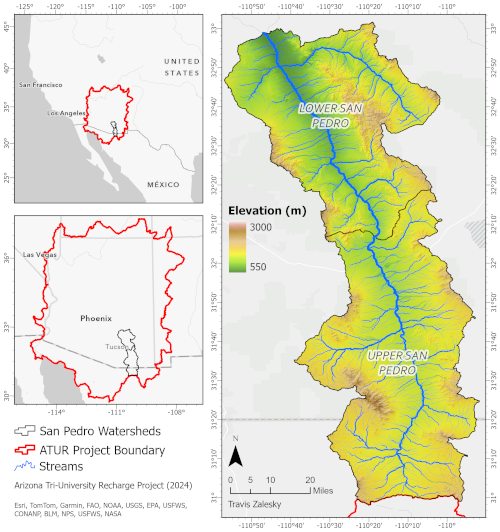
\includegraphics[keepaspectratio]{images/SanPedro_Reference_Painted.png}}

}

\caption{\label{fig-studyArea}San Pedro watershed, study area.}

\end{figure}%

\section{Data \& Methods}\label{sec-data-methods}

\subsection{Thematic Layers}\label{thematic-layers}

All data layers were processed in ArcGIS Pro v3.4.0 unless otherwise
indicated. Data layers were converted into raster data as needed, with a
30m resolution, matching the SRTM elevation raster (see
Section~\ref{sec-elev}).

\subsubsection{Elevation}\label{sec-elev}

Higher elevations are at lower flood risk due to naturally occurring
drainage, frequently in the form of surface runoff. While lower
elevations have higher surface water flow accumulation (\textbf{CITATION
NEEDED}) which can promote infiltration (\textbf{CITATION NEEDED}).

Elevation data acquired from NASA Shuttle Radar Topography Mission
(SRTM) 30m resolution global Digital Elevation Model (DEM), accessed via
Google Earth Engine (GEE) (\textbf{DATA CITATION}).

\begin{figure}

\centering{

\pandocbounded{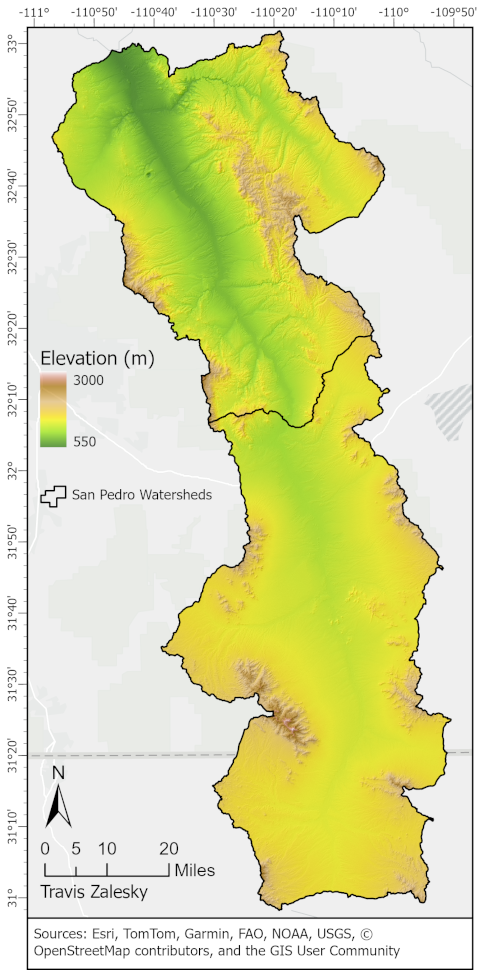
\includegraphics[keepaspectratio]{images/SanPedro_Elev.png}}

}

\caption{\label{fig-elev}San Pedro elevation 30m NASA SRTM.}

\end{figure}%

\subsubsection{Slope}\label{slope}

Steeper slopes tend to promote surface flow and high erosion. Gentler
slopes however have decreased surface water flow rates, increasing
residence time, and potentially resulting in flooding during times of
heavy rainfall or snowmelt (\textbf{CITATION NEEDED}).

Slope data was calculated as a first order derivative of the elevation
data.

\begin{figure}

\centering{

\pandocbounded{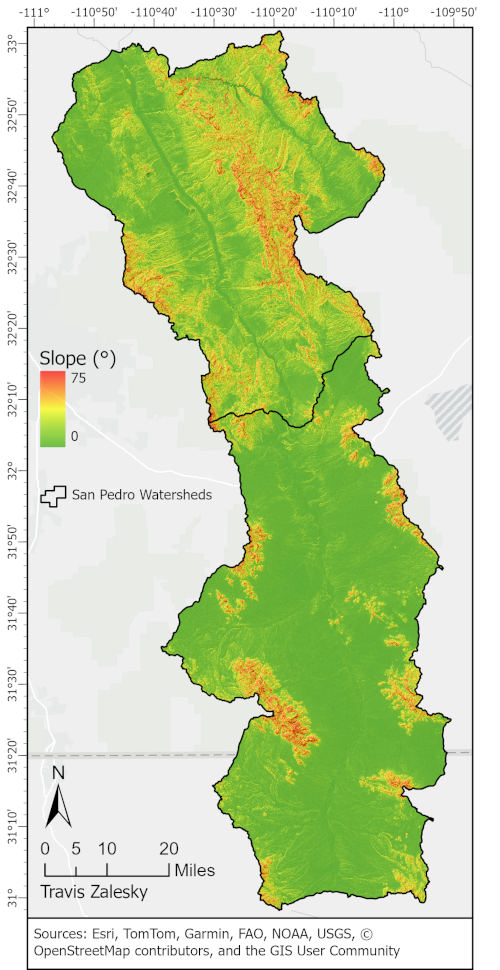
\includegraphics[keepaspectratio]{images/SanPedro_Slope.png}}

}

\caption{\label{fig-slope}San Pedro slope.}

\end{figure}%

\subsubsection{Lineament Density}\label{lineament-density}

Lineaments such as faults and fractures fundamentally influence water
flow dynamics.

\textbf{This layer is not yet available, but I believe that Ryan is
working on this concept}

See Aloui et al. (2024) section 3.1.3 Lineament density (LD) for
additional methods on generating lineament features from a DEM.

\subsubsection{Drainage Density}\label{drainage-density}

High drainage density increases flood susceptibility via rapid water
accumulation through channels (\textbf{CITATION NEEDED}). Additionally,
the increased flow rate in areas with high drainage density reduces the
residence time of surface water, limiting recharge potential
(\textbf{CITATION NEEDED}) and regions of high drainage density have
been frequently associated with less permiable soils (\textbf{CITATION
NEEDED}).

Drainage density was calculated using the USGS National Hydrography
Dataset (NHD) flowline features (\textbf{Data Citation}). This dataset
consisted of both natural and engineered flowlines, including such
things as underground pipes. Line density was calculated in Km of
flowline per Km², using a search kernel of 1 Km.

\begin{figure}

\centering{

\pandocbounded{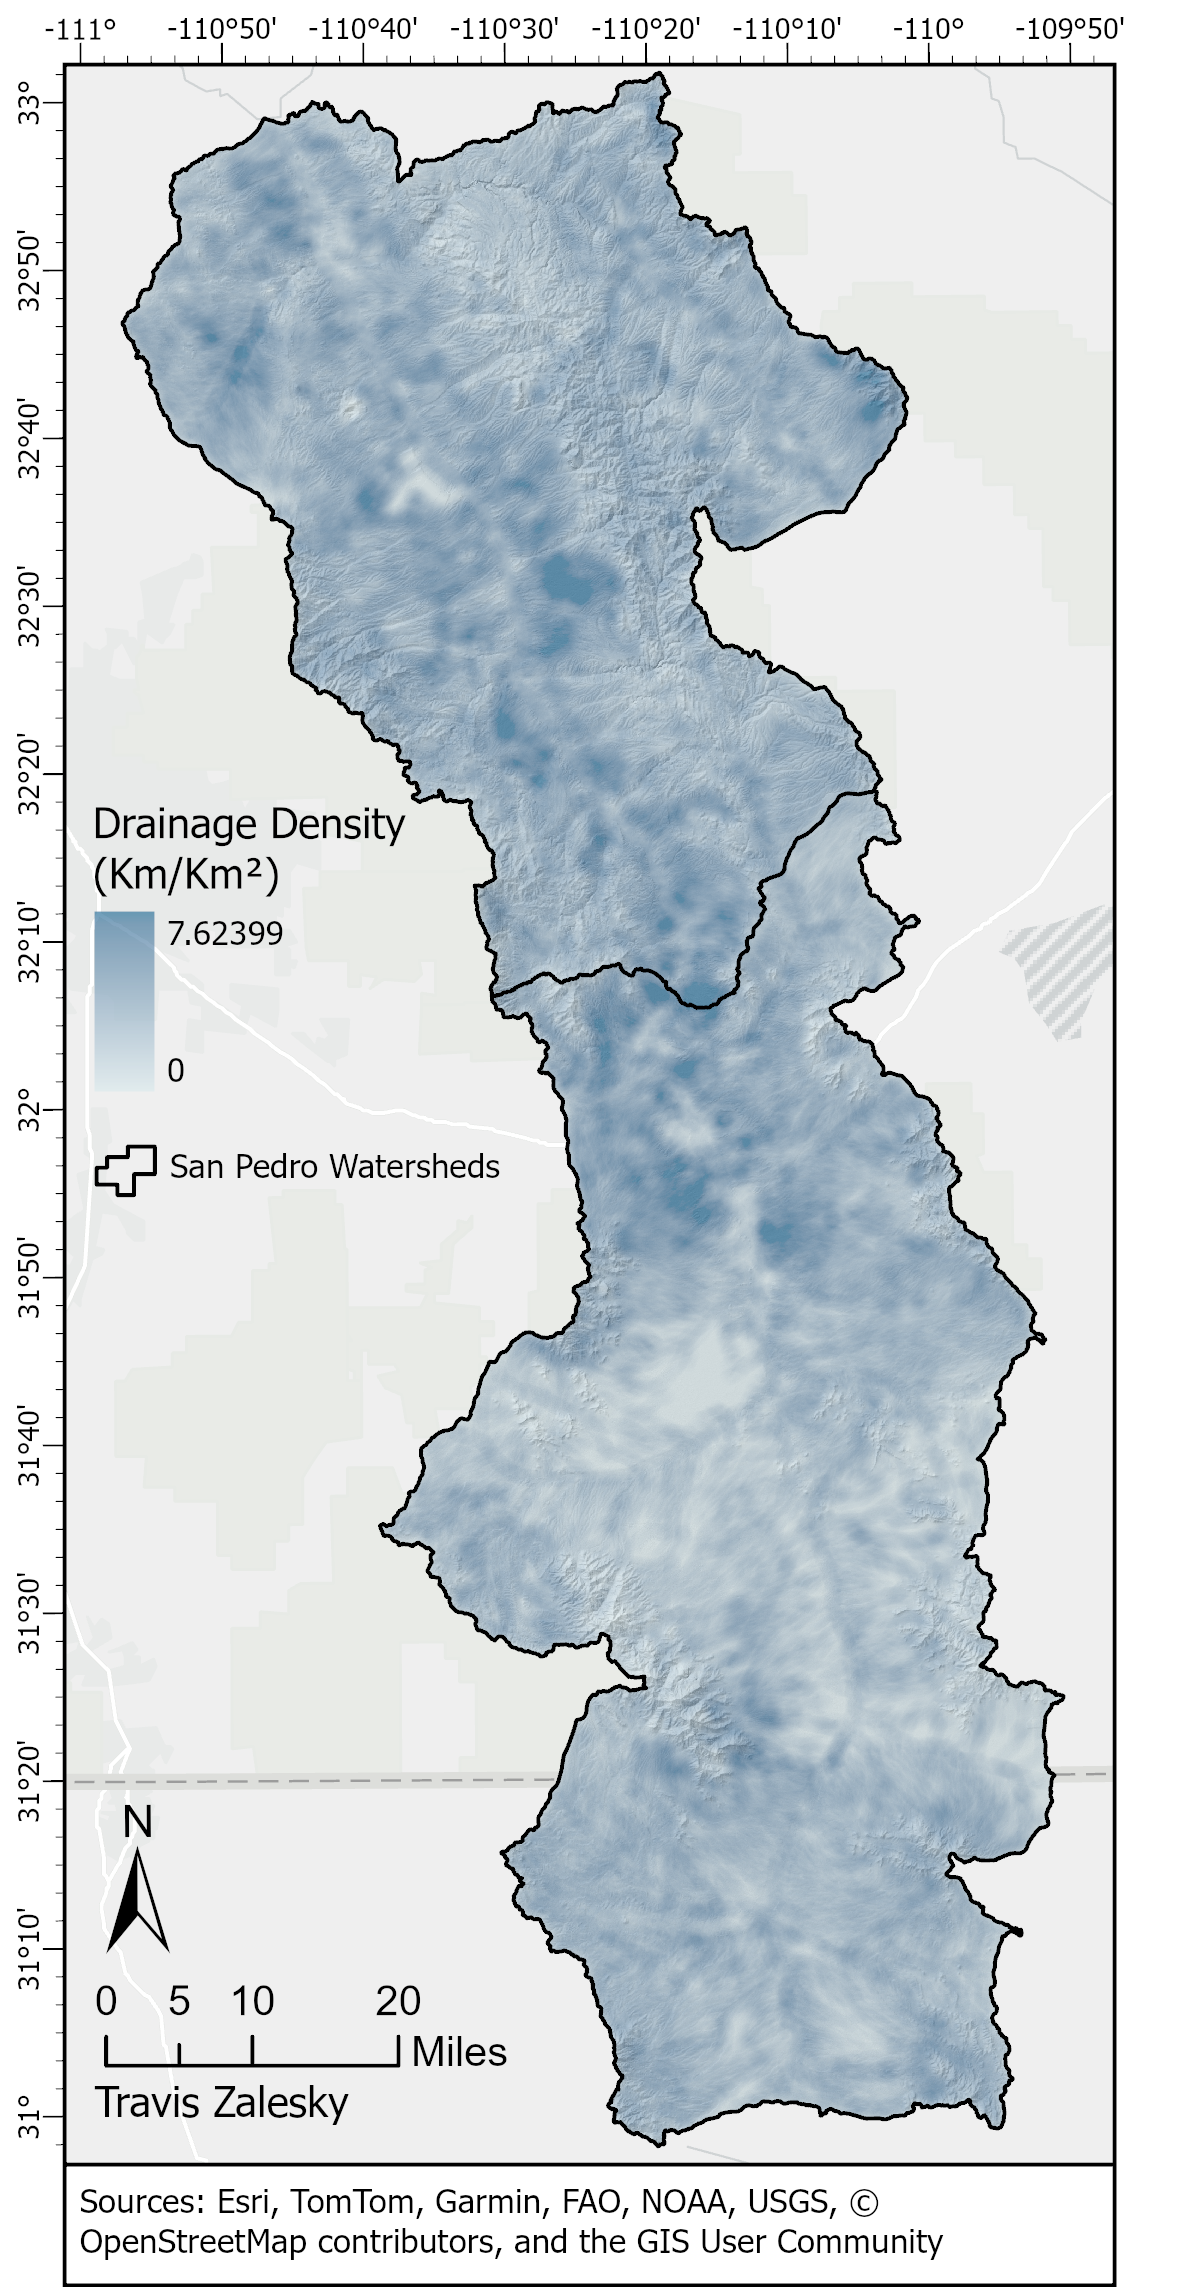
\includegraphics[keepaspectratio]{images/SanPedro_DrainDense.png}}

}

\caption{\label{fig-drain}San Pedro drainage density. Line density
calculated using a 1 Km search kernel.}

\end{figure}%

\subsubsection{Precipitation}\label{precipitation}

Precipitation is the primary source of freshwater for aquifer recharge,
as well as being the prevailing force driving regional flooding
(\textbf{CITATION NEEDED}).

Precipitation data was obtained from OSU PRISM data using 30-year
normals 800 m resolution, subsequently downscaled to match the SRTM 30 m
resolution using bilinear interpolation (\textbf{DATA CITATION}). The
PRISM dataset extends approximately 10 Km S of the US-Mexico border, but
unfortunately it does not cover the entire watershed. The extent of the
uncovered portion of the watershed is approximately 1,200 Km²,
representing roughly 12\% of the total area.

\begin{tcolorbox}[enhanced jigsaw, colframe=quarto-callout-note-color-frame, bottomrule=.15mm, left=2mm, opacitybacktitle=0.6, arc=.35mm, breakable, colbacktitle=quarto-callout-note-color!10!white, leftrule=.75mm, coltitle=black, titlerule=0mm, rightrule=.15mm, colback=white, bottomtitle=1mm, toprule=.15mm, title=\textcolor{quarto-callout-note-color}{\faInfo}\hspace{0.5em}{Note}, opacityback=0, toptitle=1mm]

\emph{In the San Pedro watershed precipitation is highly correlated with
elevation. Using a simple linear trendline across the entire watershed
elevation accounts for 51\% of the variance in precipitation, increasing
to 81\% when using an E-W transect located at the US-Mexico border (data
not shown). This corelation could potentially be leveraged to fill in
the missing data through a variety of interpolation techniques.}

\end{tcolorbox}

\begin{figure}

\centering{

\pandocbounded{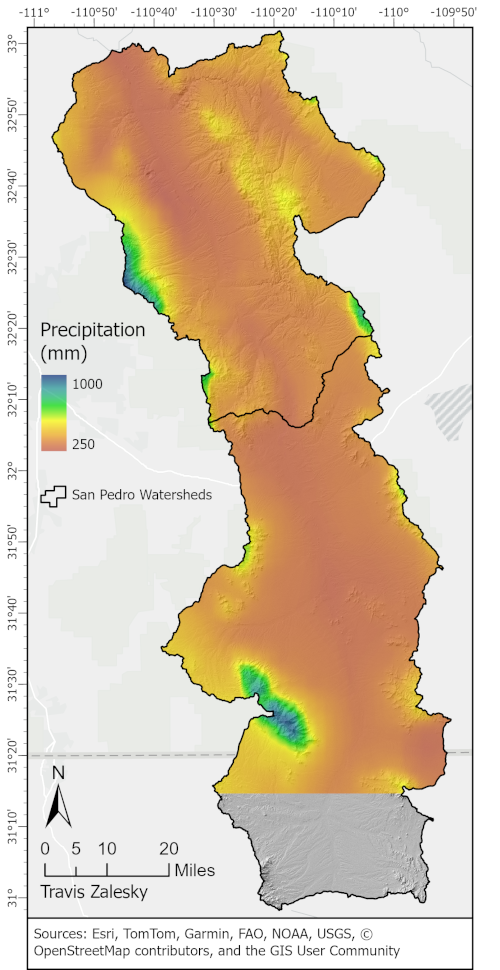
\includegraphics[keepaspectratio]{images/SanPedro_Precip.png}}

}

\caption{\label{fig-precip}San Pedro average annual precipitation.
Derived from OSU PRISM 30-year normals (800 m), downscaled to 30 m
resolution.}

\end{figure}%

\subsubsection{Lithology}\label{lithology}

The characteristics of surface rock profoundly impact recharge, as the
primary factor governing permeability (\textbf{CITATION NEEDED}).

Lithology data from the USGS State Geologic Map Compilation
(\textbf{DATA CITATION}). Depending on how the geologic units are
defined (i.e.~by ``Unit Name'', primary, secondary, tertiary lithology,
or combination) there are upwards of 25 distinct geologic units which
must be classified. The USGS SGMC terminates at the US-Mexico border,
and it is not clear if any relevant data within Mexico can be located.
The extent of the uncovered portion of the watershed is approximately
1,800 Km², representing roughly 16\% of the total area.

\paragraph{\texorpdfstring{\textbf{PLEASE
ADVISE!}}{PLEASE ADVISE!}}\label{please-advise}

\begin{longtable}[]{@{}
  >{\raggedright\arraybackslash}p{(\linewidth - 2\tabcolsep) * \real{0.6761}}
  >{\raggedright\arraybackslash}p{(\linewidth - 2\tabcolsep) * \real{0.3239}}@{}}
\toprule\noalign{}
\begin{minipage}[b]{\linewidth}\raggedright
Geologic Unit Name
\end{minipage} & \begin{minipage}[b]{\linewidth}\raggedright
Suitability Classification (1-10)
\end{minipage} \\
\midrule\noalign{}
\endhead
\bottomrule\noalign{}
\endlastfoot
Early Proterozoic granitic rocks & \\
Quaternary surficial deposits, undivided & \\
Early Proterozoic metasedimentary rocks & \\
Pliocene to middle Miocene deposits & \\
Early Tertiary to Late Cretaceous granitic rocks & \\
Middle Proterozoic diabase & \\
Cretaceous to Late Jurassic sedimentary rocks with minor volcanic rocks
& \\
Mississippian, Devonian, and Cambrian sedimentary rocks & \\
Paleozoic sedimentary rocks & \\
Early Tertiary to Late Cretaceous volcanic rocks & \\
Jurassic volcanic rocks & \\
Middle Miocene to Oligocene granitic rocks & \\
Middle Miocene to Oligocene volcanic rocks & \\
Jurassic granitic rocks & \\
Early Proterozoic metamorphic rocks & \\
Early Tertiary to Late Cretaceous muscovite-bearing granitic rocks & \\
Holocene surficial deposits & \\
Middle Miocene to Oligocene sedimentary rocks & \\
Early Pleistocene to latest Pliocene surficial deposits & \\
Middle Proterozoic sedimentary rocks & \\
Middle Proterozoic granitic rocks & \\
Permian to Pennsylvanian sedimentary rocks & \\
Jurassic sedimentary and volcanic rocks & \\
Tertiary to Early Proterozoic gneissic rocks & \\
Holocene river alluvium & \\
\end{longtable}

\begin{figure}

\centering{

\pandocbounded{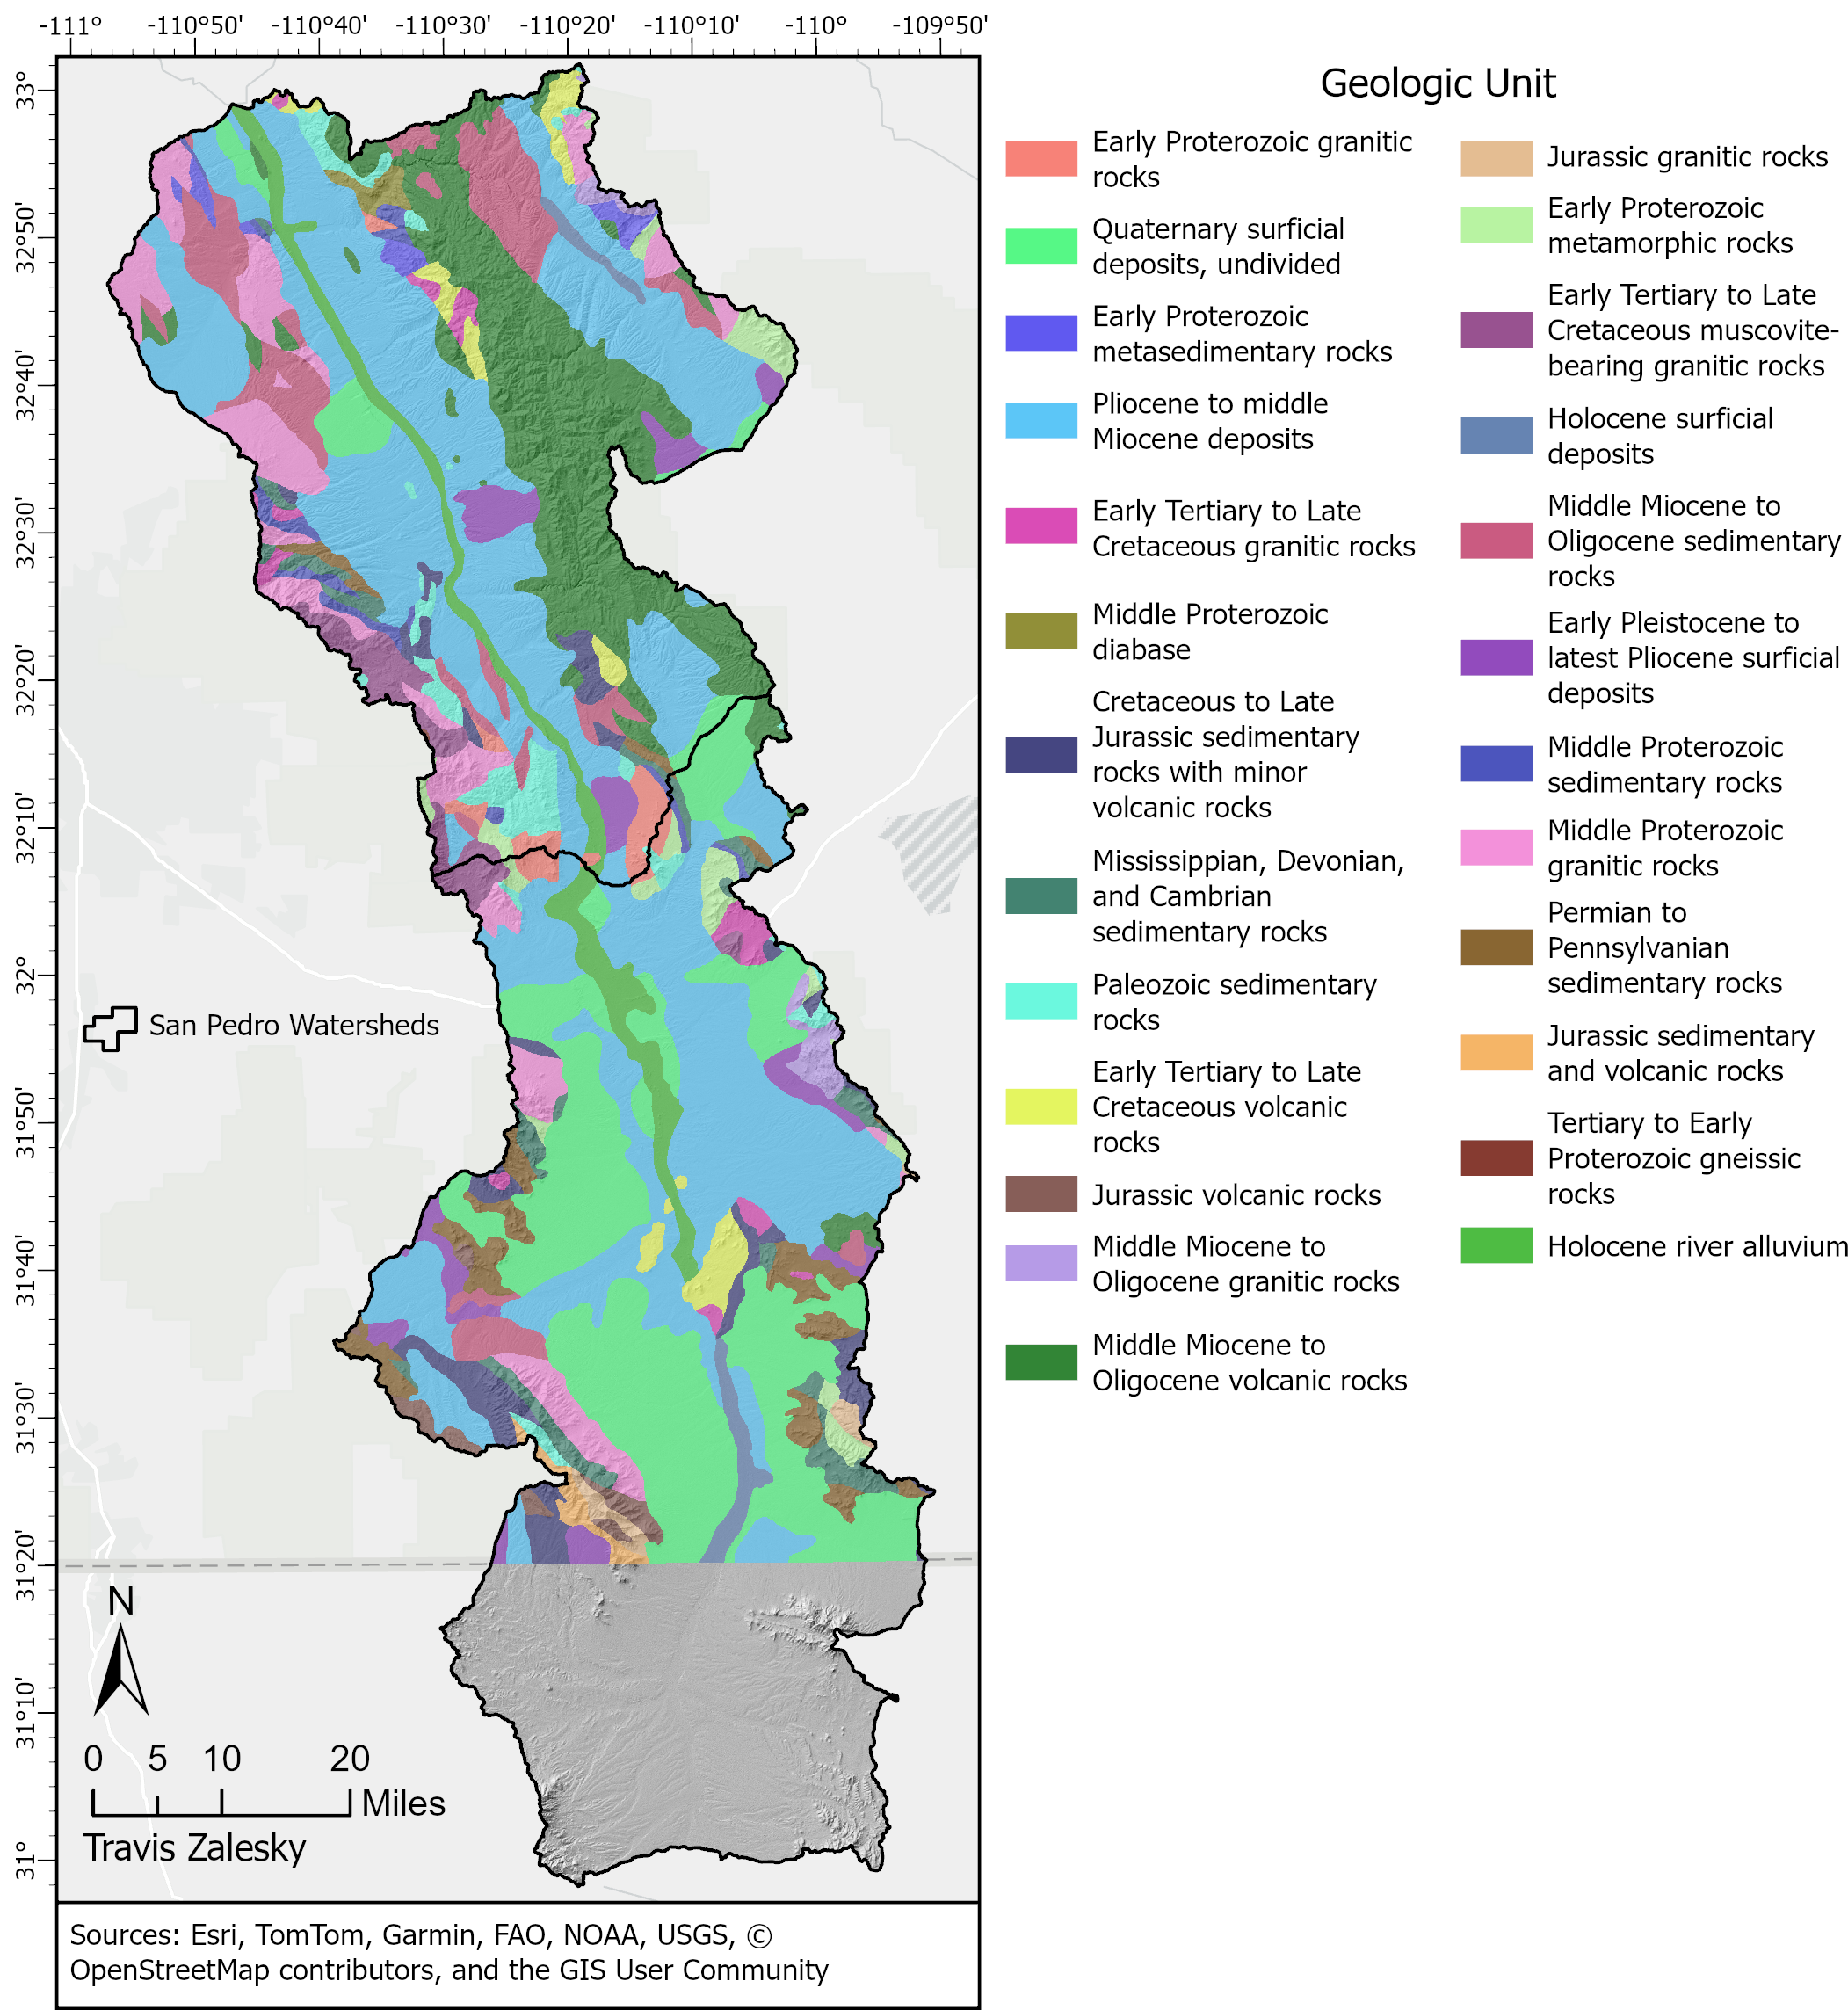
\includegraphics[keepaspectratio]{images/SanPedro_Lith.png}}

}

\caption{\label{fig-lith}San Pedro lithology.}

\end{figure}%

\subsubsection{Soil Type}\label{soil-type}

Soil texture influences infiltration via it's impacts on porosity and
adhesion (\textbf{CITATION NEEDED}). Finer soil textures increase
runoff, reducing infiltration, and visa versa (\textbf{CITATION
NEEDED}).

\textbf{Original soil data source unknown. Presumably USGS Soil
Survey(?). PLEASE ADVISE!}

Soil type is classified into 1 of 7 soil hydrologic groups\ldots{}
\emph{Additional details about classification methods}

As with the USGS lithology data, the soils data ends abruptly at the
US-Mexico border. At this time data availability within Mexico has not
been identified.

These USGS(?) classifications were assigned an additional suitability
classification ranking from 1-10 according to Table~\ref{tbl-soil}

\begin{longtable}[]{@{}
  >{\centering\arraybackslash}p{(\linewidth - 6\tabcolsep) * \real{0.1892}}
  >{\centering\arraybackslash}p{(\linewidth - 6\tabcolsep) * \real{0.1892}}
  >{\centering\arraybackslash}p{(\linewidth - 6\tabcolsep) * \real{0.4324}}
  >{\centering\arraybackslash}p{(\linewidth - 6\tabcolsep) * \real{0.1892}}@{}}
\caption{Soil hydrologic group.}\label{tbl-soil}\tabularnewline
\toprule\noalign{}
\begin{minipage}[b]{\linewidth}\centering
Class
\end{minipage} & \begin{minipage}[b]{\linewidth}\centering
Count (pixels)*
\end{minipage} & \begin{minipage}[b]{\linewidth}\centering
Text
\end{minipage} & \begin{minipage}[b]{\linewidth}\centering
Value
\end{minipage} \\
\midrule\noalign{}
\endfirsthead
\toprule\noalign{}
\begin{minipage}[b]{\linewidth}\centering
Class
\end{minipage} & \begin{minipage}[b]{\linewidth}\centering
Count (pixels)*
\end{minipage} & \begin{minipage}[b]{\linewidth}\centering
Text
\end{minipage} & \begin{minipage}[b]{\linewidth}\centering
Value
\end{minipage} \\
\midrule\noalign{}
\endhead
\bottomrule\noalign{}
\endlastfoot
A & 62559472 & Group A soils consist of deep, well drained sands or
gravelly sands with high infiltration and low runoff rates. & 10 \\
B & 76665198 & Group B soils consist of deep well drained soils with a
moderately fine to moderately coarse texture and a moderate rate of
infiltration and runoff. & 8 \\
C & 88491710 & Group C consists of soils with a layer that impedes the
downward movement of water or fine textured soils and a slow rate of
infiltration. & 5 \\
D & 155095790 & Group D consists of soils with a very slow infiltration
rate and high runoff potential. This group is composed of clays that
have a high shrink-swell potential, soils with a high water table, soils
that have a clay pan or clay layer at or near the surface, and soils
that are shallow over nearly impervious material. & 2 \\
A/D & 43192 & Group A/D soils naturally have a very slow infiltration
rate due to a high water table but will have high infiltration and low
runoff rates if drained. & 7 \\
B/D & 18456 & Group B/D soils naturally have a very slow infiltration
rate due to a high water table but will have a moderate rate of
infiltration and runoff if drained. & 6 \\
C/D & 217771 & Group C/D soils naturally have a very slow infiltration
rate due to a high water table but will have a slow rate of infiltration
if drained. & 3 \\
\end{longtable}

\emph{* Full HUC8 study area.}

\begin{figure}

\centering{

\pandocbounded{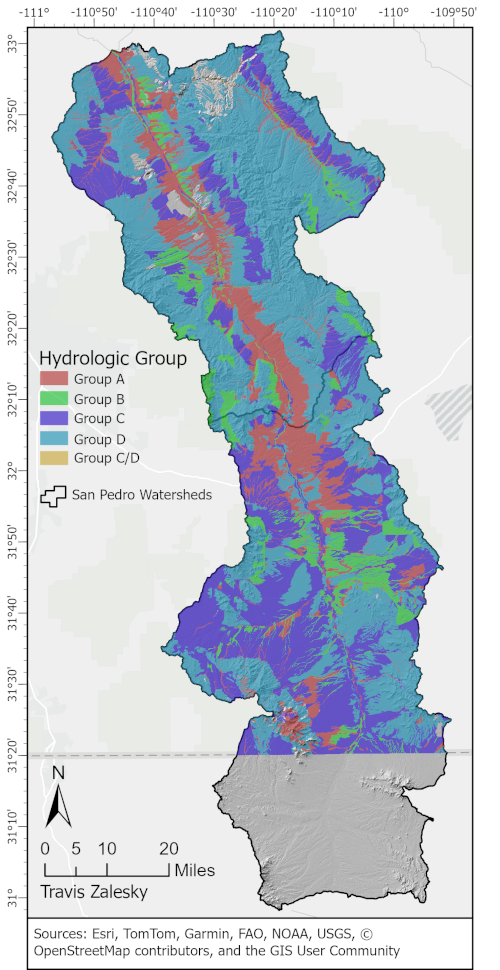
\includegraphics[keepaspectratio]{images/SanPedro_Soil.png}}

}

\caption{\label{fig-soil}San Pedro soils hydrologic group.}

\end{figure}%

\subsubsection{NDVI}\label{ndvi}

Normalized Difference Vegetation Index (NDVI) is a proxy for vegetation
health and cover. High NDVI reduces flood risk and promotes infiltration
due to vegetation's ability to reduce surface runoff flow rate, and
create macro-pores in the soil (\textbf{CITATION NEEDED}).

NDVI is a highly seasonally dependent index. To account for normal
seasonal variation, a 10-year mean NDVI was calculated using Landsat 8
and 9 imagery from early 2013 (launch of LS-8) through 2023
(\textbf{DATA CITATION}). NDVI preprocessing and analysis was carried
out in Google Earth Engine using the Javascript editor.

\begin{Shaded}
\begin{Highlighting}[]
\NormalTok{// San Pedro NDVI}
\NormalTok{// Travis Zalesky}
\NormalTok{// ATUR}
\NormalTok{// 11/14/24}
\NormalTok{// }

\NormalTok{// Import module for usefull landsat functions}
\NormalTok{var landsatFunctions = require(\textquotesingle{}users/travisz09/UsefulFunctions:LandsatFunctions\textquotesingle{})}

\NormalTok{// Study Area}
\NormalTok{print(\textquotesingle{}San Pedro\textquotesingle{}, sanPedro);}

\NormalTok{// Map setup}
\NormalTok{Map.centerObject(sanPedro, 8);}

\NormalTok{Map.addLayer(ee.Image().byte().paint(sanPedro, \textquotesingle{}black\textquotesingle{}, 2), \{\}, \textquotesingle{}San Pedro\textquotesingle{});}

\NormalTok{// Study period}
\NormalTok{var startDate = \textquotesingle{}2013{-}01{-}01\textquotesingle{};  // First year of LS{-}8}
\NormalTok{var endDate = \textquotesingle{}2024{-}01{-}01\textquotesingle{};  // Exclusive end date}

\NormalTok{// Landsat coll}
\NormalTok{var cloudFilter = 10;  // 10\% max cloud cover}
\NormalTok{var landsat  = ee.ImageCollection(\textquotesingle{}LANDSAT/LC08/C02/T1\_L2\textquotesingle{})}
\NormalTok{  // Combine Lst{-}9 and Lst{-}8}
\NormalTok{  .merge(ee.ImageCollection(\textquotesingle{}LANDSAT/LC09/C02/T1\_L2\textquotesingle{}))  }
\NormalTok{  .filterDate(startDate, endDate)}
\NormalTok{  .filterBounds(sanPedro)}
\NormalTok{  // Filter by paths and rows to return minimum images for full coverage}
\NormalTok{  .filter(ee.Filter.or(}
\NormalTok{    ee.Filter.and(}
\NormalTok{      ee.Filter.eq(\textquotesingle{}WRS\_PATH\textquotesingle{}, 35),}
\NormalTok{      ee.Filter.eq(\textquotesingle{}WRS\_ROW\textquotesingle{}, 37)),}
\NormalTok{    ee.Filter.and(}
\NormalTok{      ee.Filter.eq(\textquotesingle{}WRS\_PATH\textquotesingle{}, 35),}
\NormalTok{      ee.Filter.eq(\textquotesingle{}WRS\_ROW\textquotesingle{}, 38)),}
\NormalTok{    ee.Filter.and(}
\NormalTok{      ee.Filter.eq(\textquotesingle{}WRS\_PATH\textquotesingle{}, 36),}
\NormalTok{      ee.Filter.eq(\textquotesingle{}WRS\_ROW\textquotesingle{}, 37))))}
\NormalTok{  .sort(\textquotesingle{}system:time\_start\textquotesingle{})  // Sort by date}
\NormalTok{  // .filter(ee.Filter.lt(\textquotesingle{}CLOUD\_COVER\textquotesingle{}, cloudFilter));}
\NormalTok{  .map(landsatFunctions.renameL8)  // Rename bands}
  
\NormalTok{print(\textquotesingle{}Landsat Collection\textquotesingle{}, landsat);}
\NormalTok{Map.addLayer(ee.Image().byte().paint(landsat.limit(3),}
\NormalTok{ \textquotesingle{}blue\textquotesingle{}, 1), \{\}, \textquotesingle{}Landsat\textquotesingle{})}


\NormalTok{landsat = landsat.map(landsatFunctions.addMask)}

\NormalTok{var NDVI = landsat.map(function(img) \{}
\NormalTok{  var ndvi = img.normalizedDifference([\textquotesingle{}NIR\textquotesingle{}, \textquotesingle{}RED\textquotesingle{}])}
\NormalTok{    .rename(\textquotesingle{}ndvi\textquotesingle{});}
  
\NormalTok{  return img.addBands(ndvi)}
\NormalTok{\})}

\NormalTok{Map.addLayer(NDVI.select(\textquotesingle{}ndvi\textquotesingle{}).limit(3), \{}
\NormalTok{  min: 0,}
\NormalTok{  max: 0.4,}
\NormalTok{  palette: [\textquotesingle{}red\textquotesingle{}, \textquotesingle{}yellow\textquotesingle{}, \textquotesingle{}green\textquotesingle{}]}
\NormalTok{\}, \textquotesingle{}NDVI\textquotesingle{}, false)}

\NormalTok{var meanNDVI = NDVI.select(\textquotesingle{}ndvi\textquotesingle{}).mean()}

\NormalTok{meanNDVI = meanNDVI.clip(sanPedro);}

\NormalTok{print(\textquotesingle{}Mean NDVI\textquotesingle{}, meanNDVI)}
\NormalTok{Map.addLayer(meanNDVI, \{}
\NormalTok{  min: 0,}
\NormalTok{  max: 0.3,}
\NormalTok{  palette: [\textquotesingle{}red\textquotesingle{}, \textquotesingle{}yellow\textquotesingle{}, \textquotesingle{}green\textquotesingle{}]}
\NormalTok{\}, \textquotesingle{}Mean NDVI\textquotesingle{})}

\NormalTok{Export.image.toDrive(\{}
\NormalTok{  image: meanNDVI, }
\NormalTok{  description: \textquotesingle{}SanPedroNDVI\_10yrMean\textquotesingle{},}
\NormalTok{  folder: \textquotesingle{}ATUR/Data\textquotesingle{},}
\NormalTok{  fileNamePrefix: \textquotesingle{}SanPedroNDVI\_10yrMean\textquotesingle{},}
\NormalTok{  region: sanPedro,}
\NormalTok{  scale: 30,}
\NormalTok{  crs: \textquotesingle{}EPSG:32612\textquotesingle{}}
\NormalTok{\})}
\end{Highlighting}
\end{Shaded}

\begin{figure}

\centering{

\pandocbounded{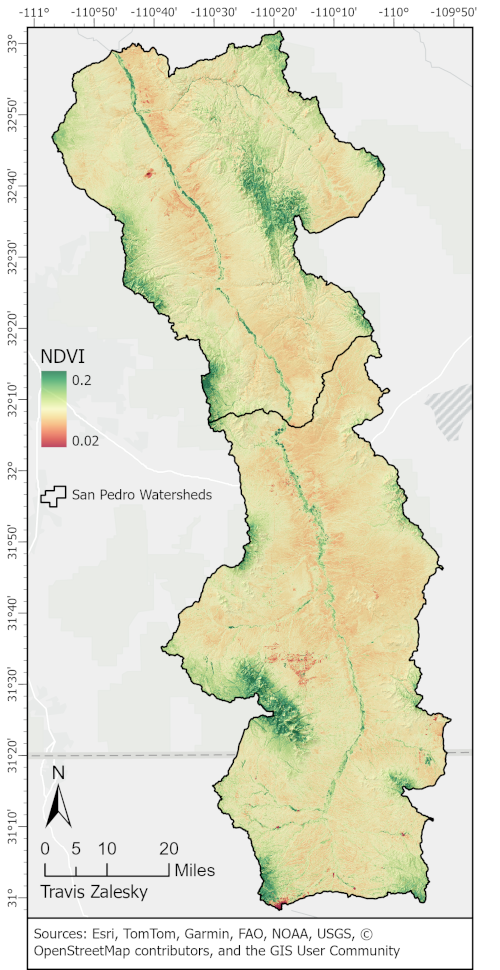
\includegraphics[keepaspectratio]{images/SanPedro_NDVI.png}}

}

\caption{\label{fig-ndvi}San Pedro 10-year mean NDVI.}

\end{figure}%

\subsubsection{Land use/land cover}\label{land-useland-cover}

Infiltration and runoff rates are highly influenced by land cover
(\textbf{CITATION NEEDED}). ESRI 2020 Global Land Use Land Cover from
Sentinel-2 (ESRI LULC) is a 10-m resolution global land cover dataset
derived from proprietary machine-learning algorithm run on Sentinel-2
satellite imagery (\textbf{DATA CITATION}). ESRI LULC was accessed and
clipped to the study area using Google Earth Engine. The pixel
resolution was reduced to 30 m.

\begin{Shaded}
\begin{Highlighting}[]
\NormalTok{// Land Use Land Cover}
\NormalTok{// Travis Zalesky}
\NormalTok{// ATUR}
\NormalTok{// 11/14/24}

\NormalTok{var studyArea = ee.FeatureCollection("projects/ee{-}travisz09/assets/ATUR/WBDHU8\_OuterBoundary\_Project");}

\NormalTok{var esri\_lulc10 = ee.ImageCollection("projects/sat{-}io/open{-}datasets/landcover/ESRI\_Global{-}LULC\_10m")}
\NormalTok{  .filterBounds(studyArea)}
\NormalTok{  .mosaic()}
\NormalTok{  .clip(studyArea);}
  
\NormalTok{print(esri\_lulc10)}

\NormalTok{Export.image.toDrive(\{}
\NormalTok{  image: esri\_lulc10, }
\NormalTok{  description: \textquotesingle{}ESRI\_LULC\_10m\_mergedClipped\textquotesingle{},}
\NormalTok{  folder: \textquotesingle{}ATUR/Data\textquotesingle{},}
\NormalTok{  fileNamePrefix: \textquotesingle{}ESRI\_LULC\_10m\_clip\textquotesingle{},}
\NormalTok{  region: studyArea,}
\NormalTok{  scale: 30,}
\NormalTok{  crs: \textquotesingle{}EPSG:32612\textquotesingle{},}
\NormalTok{  maxPixels: 1e12}
\NormalTok{\})}
\end{Highlighting}
\end{Shaded}

\subsubsection{Stormwater Drainage
Density}\label{stormwater-drainage-density}

\textbf{I am unaware of any data availability for this layer. PLEASE
ADVISE!}

\section{Conclusion}\label{conclusion}

\section*{References}\label{references}
\addcontentsline{toc}{section}{References}

\phantomsection\label{refs}
\begin{CSLReferences}{1}{0}
\vspace{1em}

\bibitem[\citeproctext]{ref-aloui2024}
Aloui, S., Zghibi, A., Mazzoni, A., Elomri, A., \& Al-Ansari, T. (2024).
Identifying suitable zones for integrated aquifer recharge and flood
control in arid qatar using GIS-based multi-criteria decision-making.
\emph{Groundwater for Sustainable Development}, \emph{25}, 101137.
\url{https://doi.org/10.1016/j.gsd.2024.101137}

\end{CSLReferences}




\end{document}
